\documentclass{article}
% [landscape]
\usepackage{amsmath, amsthm, amssymb, bm, color, framed, graphicx, hyperref, mathrsfs}
\usepackage{graphicx}%图片头文件
\usepackage{float} %指定图片位置
\usepackage{subfigure}%并排子图 共享标题 有子标题
\usepackage{caption}
\usepackage[margin=1in,letterpaper]{geometry} 

% code
\usepackage{listings} 
\usepackage{xcolor}
\lstset{
  language=Matlab,  %代码语言使用的是matlab
  frame=shadowbox, %把代码用带有阴影的框圈起来
  rulesepcolor=\color{red!20!green!20!blue!20},%代码块边框为淡青色
  keywordstyle=\color{blue!90}\bfseries, %代码关键字的颜色为蓝色,粗体
  commentstyle=\color{red!10!gray!70}\textit,    % 设置代码注释的颜色
  showstringspaces=false,%不显示代码字符串中间的空格标记
  numbers=left, % 显示行号
  numberstyle=\tiny,    % 行号字体
  stringstyle=\ttfamily, % 代码字符串的特殊格式
  breaklines=true, %对过长的代码自动换行
  extendedchars=false,  %解决代码跨页时,章节标题,页眉等汉字不显示的问题
%   escapebegin=\begin{CJK*},escapeend=\end{CJK*},      % 代码中出现中文必须加上,否则报错
  texcl=true}


\usepackage{ctex}
\usepackage{amsmath}
\usepackage{graphicx}
\usepackage{epstopdf}
\usepackage{tikz}
\usepackage{psfrag}
\usepackage{natbib}
\usepackage{hyperref}

\begin{document}

\renewcommand{\refname}{参考文献}
\renewcommand{\figurename}{图}
\renewcommand{\abstractname}{摘要}
\def\due{2022 年 3 月 7 日周一 8:40}

\title{《磁流体力学的数值模拟方法》-- 第4次作业 \footnote{2022 春季《磁流体力学的数值模拟方法》}}


\author{蓝翔\footnote{Email: shsxjujishou@163.com
, 学号: SA21214038}
\and
康樨\footnote{Email: kx\_0045@mail.ustc.edu.cn, 学号: SA21007083}
\and
苏镇波\footnote{Email: zbsu@mail.ustc.edu.cn, 学号: SA21022002}
}

\date{%
\scriptsize%
%CAS Key Laboratory for Basic Plasma Physics, School of Earth and Space Sciences,
%\\
%University of Science and Technology of China, Hefei, Anhui 230026, China
中国科学技术大学核科学技术学院,合肥 230026\\
中国科学技术大学地球与空间科学学院, 合肥 230026\\
中国科学技术大学物理学院天文系, 合肥 230026
%
}

\maketitle

\begin{abstract}
讨论一维磁流体力学 (MHD, Magnetohydrodynamics) 激波问题的有限
差分数值解法, 结合理论分析讨论磁声波的特性, 分析较弱激波以及快、慢激波的计算.

\end{abstract}

\section{引言}
理想磁流体力学激波是指在理想磁流体力学条件下(无耗散,无电阻)情况下产生的一种非线性现象。当流速大于同方向扰动传播速度时,流体可压缩性会使流体形态发生突变,产生时空上高度非线性的激波。这时在高速推进的初始上游流体和被它推动的下游流体间会出现一层以上游流速向前推进的、陡立的波前。而波前中,流体状态量会从上游的取值开始,经过急剧的空间变化过渡到下游取值。激波中,波前运动特征时间尺度和状态量变化特征空间尺度都比上下游状态量的时空变化特征尺度短得多。
\par
本文将研究在一定初始条件下强弱激波中各物理量空间分布随时间的发展变化,分析激波的发展趋势,并和经典文献结果进行对比以观察我们所得的数值结果特点。
\section{一维磁流体力学激波\citep{Jeffrey1964}}
守恒型方程
\begin{align}
\frac{\partial U}{\partial t} + \nabla \cdot \boldsymbol{F} &= 0. \label{Eqn:3.1.6}
\end{align}
间断两侧满足关系
\begin{align}
[\tilde{\lambda} U - \boldsymbol{F} \cdot \boldsymbol{n}_1] &= 0 \label{Eqn:3.1.11}
\end{align}
或者
\begin{align}
\tilde{\lambda} [U] &= [\boldsymbol{F} \cdot \boldsymbol{n}_1]. \label{Eqn:3.1.11a}
\end{align}
其中 $\tilde{\lambda}$ 是间断移动的速度, $\boldsymbol{n}_1$ 为间断面的单位法向量.

对一维磁流体, 设所有的物理量只是 $x$ 和 $t$ 的函数,
\begin{align}
U_t + F_x &= 0 \label{Eqn:6.1.1}
\end{align}
这里
\begin{align}
U &= \left[\begin{array}{c}
\rho \\
\rho v_x \\
\frac{1}{2} \rho v^2 + \rho e + p_m \\
\rho v_y \\
H_y \\
\rho v_z \\
H_z
\end{array}\right], \label{Eqn:6.1.2a}
\\
F &= \left[\begin{array}{l}
\rho v_x \\
\rho v_x^2 + p^* \\
v_x \left( \frac{\rho v^2}{2} + \rho e + p_m \right) + v_x p^* - \frac{\mu}{4\pi} H_x \boldsymbol{v} \cdot \boldsymbol{H} \\
\rho v_y v_x - \frac{\mu}{4\pi} H_x H_y \\
H_y v_x - v_y H_x \\
\rho v_z v_x - \frac{\mu}{4\pi} H_x H_z \\
H_z v_x - v_z H_x
\end{array}\right]. \label{Eqn:6.1.2b}
\end{align}
其中 $\rho$, $p$, $e$, $\boldsymbol{v} = (v_x, v_y, v_z)$, 和 $\boldsymbol{H} = (H_x, H_y, H_z)$ 分别是密度, 压强, 内能, 速度, 和磁场. $p_m = \mu H^2/8\pi$ 为磁压, $p^* = p + p_m$ 为总压强. 由磁场无散条件 $\nabla \cdot \boldsymbol{H} = 0$, $H_x$ 是常数, 公式~(\ref{Eqn:3.1.11a}) 因此化为
\begin{align}
\left[ \rho \tilde v_x \right] &= 0 \label{Eqn:6.1.3}
\\
\left[ \rho v_x \tilde v_x + p^* \right] &= 0
\\
\left[\tilde v_x \left( \frac{\rho}{2} v^2 + \rho e + \frac{\mu}{8\pi} H^2 \right) +
v_x p^* -
\frac{\mu}{4\pi} H_x \boldsymbol{v} \cdot \boldsymbol{H} \right] &= 0 \label{Eqn:6.1.6}
\\
\left[ \rho v_y \tilde v_x - \frac{\mu}{4\pi} H_x H_y \right] &= 0
\\
\left[ \tilde v_x H_y - H_x v_y \right] &= 0 \label{Eqn:6.1.8}
\\
\left[ \rho v_z \tilde v_x - \frac{\mu}{4\pi} H_x H_z \right] &= 0
\\
\left[ \tilde v_x H_z - H_x v_z \right] &= 0 \label{Eqn:6.1.10}
\end{align}
此处 $\tilde v_x$ 相对于间断流体速度的 $x$ 分量, 即
\begin{align}
\tilde v_x = v_x - \tilde\lambda
\end{align}
假设 $\tilde\lambda$ 为常数. 使用随间断运动的坐标系,
在这个坐标系中速度 $\boldsymbol{v}' = (v_x', v_y', v_z')$, 磁场 $\boldsymbol{H'} = (H_x', H_y',
H_z')$. Galilean 变换的结果是 $\boldsymbol{H}$ 不变, 速度由下面方程决定
\begin{align*}
v_x' = & v_x - \tilde\lambda = \tilde v_x \\
v_y' = & v_y \\
v_z' = & v_z. 
\end{align*}
在不造成混淆的情况下, 直接用 $\boldsymbol{v} = (v_x, v_y, v_z)$ 和 $\boldsymbol{H} = (H_x, H_y, H_z)$ 表示 ${\bf
v'}$ 和 $\boldsymbol{H}'$. 将间断位置设为坐标原点, 即
\begin{align*}
x &= 0.
\end{align*}
定义
\begin{align*}
\left<Q\right> &= \frac{1}{2}(Q_0 + Q_1),
\end{align*}
角标 0 和 1 分别表示间断两侧 (波前/上游和波后/下游) 的量. 进而可以将跃变关系~(\ref{Eqn:6.1.3})-(\ref{Eqn:6.1.10}) 表示为
\begin{align}
m[\tau] - [v_x] &= 0 \label{Eqn:6.1.4a}
\\
m[v_x] + [p] + \frac{\mu}{4\pi} \left< \bf H \right> \cdot [\bf H ] &=
0\label{Eqn:6.1.5a}
\\
m[v_y] - \frac{\mu}{4\pi} H_x [H_y] &= 0\label{Eqn:6.1.7a}
\\
m \left<\tau \right> [H_y] + \left< H_y \right> [v_x] - H_x [v_y] &= 0\label{Eqn:6.1.8a}
\\
m [v_z] - \frac{\mu}{4\pi} H_x [H_z] &= 0
\\
m \left< \tau \right> [H_z] - H_x [v_z] &= 0\label{Eqn:6.1.10a}
\end{align}
这里 
\begin{align}
  \tau &= \rho^{-1},
  \\
  m &= \rho_1 \tilde v_{x1} = \rho_0 \tilde v_{x0}.
\end{align}
同时选取坐标系使得 $\left< H_z \right> = 0$. 这样, 很容易得到关于 $m$
(或者激波速度 $\tilde\lambda$) 的方程 (力学关系), 快慢磁声激波情况下为
\begin{align}
(m^2 + [\tau]^{-1}[p]) \left( m^2 - \left<\tau\right>^{-1} \frac{\mu H_x^2}{4\pi} \right)
&= m^2 \left<\tau\right>^{-1} \frac{\mu}{4\pi}
\left<H_y\right>^2\label{Eqn:6.1.13}
\end{align}
横波 (Alfven 波) 情况下为,
\begin{align}
\left<\tau\right> m^2 - \frac{\mu H_x^2}{4\pi} = 0.\label{Eqn:6.1.14}
\end{align}
能量方程~(\ref{Eqn:6.1.6}) 可以改写为,
\begin{align}
m \Bigg\{ \left[ e + \frac{\mu}{8\pi} \tau H^2 \right] +& [\tau] \left( \left<p\right>
+
\frac{\mu}{8\pi} \left<\bf H_t^2\right> - \frac{\mu}{8\pi} H_x^2 \right)
\nonumber\\
-& \frac{\mu}{4\pi} [\tau \bf H_t] \cdot \left< \boldsymbol{H}_t \right> \Bigg\} = 0
\end{align}
此处 $\boldsymbol{H}_t$ 是横向磁场
\begin{eqnarray*}
\boldsymbol{H}_t = \boldsymbol{H} - (\boldsymbol{H} \cdot \boldsymbol{n}_1) \boldsymbol{n}_1.
\end{eqnarray*}
最后得到
\begin{align}
m = 0\label{Eqn:6.1.6aa}
\end{align}
或
\begin{align}
[e] + \left<p\right>[\tau] = -\frac{\mu}{16\pi} [\tau][\bf H_t]^2.\label{Eqn:6.1.6ba}
\end{align}
(\ref{Eqn:6.1.6ba}) 称为广义 Rankine-Hugoniot 关系. (\ref{Eqn:6.1.6aa}) 为接触间断条件.

结合方程~(\ref{Eqn:6.1.13}), (\ref{Eqn:6.1.14}) 和 (\ref{Eqn:6.1.6aa}),
将磁流体力学间断分为快慢激波, 横向间断(激波)和接触间断.

不失一般性, 我们可以选取坐标系使得激波前 $H_x > 0$, $H_{y0} > 0$, 且假定 $x$ 轴指向 $\boldsymbol{n}$ 的正方向, $\boldsymbol{n}$ 为激波前指向激波后的单位向量,
即流体流入的方向. 整理后, 可将快慢磁声激波关系表示为
\begin{align}
\bar{\eta} &= h\left\{\frac{-\frac{1}{2}\gamma h \sin\theta_0 -
(1-s_0) \pm
\sqrt{R(h)}}{2 s_0 \sin\theta_0 - (\gamma-1) h}\right\},\label{Eqn:6.2.15}
\\
\bar{Y} &= \frac{\gamma}{s_0} \left\{-\frac{1}{2} h^2 +
h\left(\frac{\frac{1}{2}\gamma h \sin\theta_0 - (1-s_0) \pm
\sqrt{R(h)}}{2 s_0 \sin\theta_0 - (\gamma-1) h}\right)\right\}\label{Eqn:6.2.16a}
\\
&= \frac{\gamma}{s_0} \left\{-\frac{1}{2} h^2 +
h\left(\frac{\bar{\eta}/h - \sin\theta_0}{1 - (\bar{\eta}/h)
\sin\theta_0}\right)\right\},\label{Eqn:6.2.16b}
\end{align}
$\bar{\eta}$, $\eta$. $h$, $\bar{Y}$, $\theta_0$, $s_0$ 和 $R$ 的定义如下,
\begin{align}
\bar{\eta} &= \frac{[\rho]}{\rho_0}, \qquad \eta = \frac{\rho_1}{\rho_0} = 1 + \bar{\eta} \nonumber\\
h &= \frac{[H_y]}{H_0}, \qquad H_j = \sqrt{H_x^2+H_{yj}^2} \qquad (j=0,1) \nonumber\\
\bar{Y} &= \frac{[p]}{p_0}, \qquad Y = \frac{p_1}{p_0} = 1 + \bar{Y} \nonumber\\
s_j &= \frac{\gamma p_j}{(\mu/4\pi)H_j^2} \qquad (j=0,1) \nonumber\\
\sin\theta_j &= \frac{H_{yj}}{H_j}, \qquad 0^\circ < \theta_j < 90^\circ \qquad (j=0,1) \nonumber\\
R(h) &= h^2[\frac{1}{4} \gamma^2 \sin^2\theta_0 - (\gamma-1)] + h\sin\theta_0
(2-\gamma)(1+s_0)
\nonumber\\
& \quad + 4s_0 \sin^2\theta_0 + (1-s_0)^2.\label{Eqn:6.2.17}
\end{align}
此外
\begin{equation}
\frac{\tilde{v}_{x1}}{b_{x1}} = \eta^{\frac{1}{2}} \frac{\tilde{v}_{x0}}{b_{x0}} =
\frac{1}{[1-(\bar{\eta}/h) \sin\theta_0]^{1/2}}
\end{equation}
从而可以直接求得激波速度 $\tilde{\lambda}$ ($=v_{x0}-\tilde{v}_{x0}$).

$[v_y]$ 表示为
\begin{align}\label{Eqn:6.2.18a}
\frac{[v_y]}{b_{x1}} = \frac{b_{x1} h}{\tilde{v}_{x1} \cos\theta_0} =
\frac{h}{\cos\theta_0} \left[1 - \left(\frac{\bar{\eta}}{h}\right)
\sin\theta_0\right]^{1/2}.
\end{align}
给定 $h$ 和激波前状态, 我们可以确定激波速度以及激波后的态. 用 $v_n$, $\tilde{v}_n$ 和 $H_n$ 取代 $v_x$, $\tilde v_x$ 和 $H_x$,
可以得到不依赖于 $x$ 轴选择的一般形式. 对于 (1 型) 快磁声激波和慢激波, 激波上下游的关系式如下文所述.

\subsection{慢激波}
\begin{align}
h_s &= -\frac{[H_y]}{H_0}, \quad 0 \le h_s \le \sin\theta_0 \quad (0 < \theta_0 < 90^\circ)
\\
\bar{\eta}_s &= h_s \left\{\frac{(1-s_0) - \frac{1}{2} \gamma h_s \sin\theta_0 +
\sqrt{R^+ (h_s)}}{(\gamma-1) h_s + 2 s_0 \sin\theta_0}\right\}
\\
\bar{Y}_s &= \frac{\gamma}{s_0} \left\{-\frac{h_s^2}{2} + h_s \left[\frac{(1-s_0) +
\frac{1}{2} \gamma h_s \sin\theta_0 + \sqrt{R^+ (h_s)}}{(\gamma-1) h_s + 2
\sin\theta_0}\right]\right\}
\\
\frac{\tilde{v}_{n1}^s}{b_{n1}^s} &= \frac{1}{\eta_s^{1/2}}
\frac{\tilde{v}_{n0}^s}{b_{n0}^s} = \frac{1}{[1+(\bar{\eta}_s/h_s)\sin\theta_0]^{1/2}}
\\
\frac{[v_n^s]}{b_{n1}^s} &= - \bar{\eta}_s \frac{\tilde{v}_{n1}^s}{b_{n1}^s} =
-\frac{\bar{\eta}_s}{[1+(\bar{\eta}_s/h_s)\sin\theta_0]^{1/2}}
\\
\frac{[v_y^s]}{b_{n1}^s} &= - \frac{b_{n1}^s}{\tilde{v}_{n1}^s}
\frac{h_s}{\cos\theta_0} = -\frac{h_s}{\cos\theta_0}
[1+(\bar{\eta}_s/h_s)\sin\theta_0]^{1/2}
\\
R^+(h_s) &= h_s^2 [\frac{1}{4} \gamma^2 \sin^2\theta_0 - (\gamma-1)] - h_s \sin\theta_0
(2-\gamma)(1+s_0) \nonumber
\\
& \quad + 4s_0 \sin^2\theta_0 + (1-s_0)^2
\end{align}


\subsection{1 型快激波}
\begin{align}
h_f &= \frac{[H_y]}{H_0}
\\
s_0 &\ge 1 - \frac{\gamma}{\gamma-1} \sin^2\theta_0, \quad 0 < h_f \le \hat{\hat{h}}_f
\quad \left(\hat{\hat{h}}_f = \frac{2}{\gamma-1} \sin\theta_0\right)
\\
\bar{\eta}_f &= h_f \left\{\frac{-\frac{1}{2} \gamma h_f \sin\theta_0 - (1-s_0) +
\sqrt{R(h_f)}}{2s_0 \sin\theta_0 - (\gamma-1) h_f}\right\}, \nonumber\\
& \qquad \bar{\eta}_{f\max} = \frac{2}{\gamma-1}
\\
\bar{Y}_f &= \frac{\gamma}{s_0} \left\{-\frac{1}{2} h_f^2 + h_f \frac{-\frac{1}{2}
\gamma h_f \sin\theta_0 - (1-s_0) + \sqrt{R(h_f)}}{2s_0 \sin\theta_0 - (\gamma-1)
h_f}\right\}, \nonumber
\\
&= \frac{\gamma}{s_0} \left\{-\frac{1}{2} h_f^2 + h_f \frac{(\bar{\eta}_f/h_f) -
\sin\theta_0}{1 - (\bar{\eta}_f/h_f)\sin\theta_0}\right\}, \quad \bar{Y}_{f\max} = \infty
\\
\frac{\tilde{v}_{n1}^f}{b_{n1}^f} &= \eta_f^{-1/2} \frac{\tilde{v}_{n0}^f}{b_{n0}^f} =
\frac{1}{[1 - (\bar{\eta}_f/h_f) \sin\theta_0]^{1/2}}
\\
\frac{[v_n^f]}{b_{n1}^f} &= - \bar{\eta}_f \frac{\tilde{v}_{n1}^f}{b_{n1}^f} =
-\frac{\bar{\eta}}{[1 - (\bar{\eta}_f/h_f) \sin\theta_0]^{1/2}}
\\
\frac{[v_y^f]}{b_{n1}^f} &= \frac{b_{n1}^f}{\tilde{v}_{n1}^f} \frac{h_f}{\cos\theta_0}
= \frac{h_f}{\cos\theta_0} \left[1 - \left(\frac{\bar{\eta}_f}{h_f}\right)
\sin\theta_0\right]^{1/2}
\\
R(h_f) &= h_f^2 \left[\frac{1}{4} \gamma^2 \sin^2\theta_0 - (\gamma - 1)\right] + h_f
\sin\theta_0 (2 - \gamma) (1 + s_0)
\nonumber\\
& \quad + 4s_0 \sin^2\theta_0 + (1 - s_0)^2
\end{align}

\section{数值方法简述}
Lax-Wendroff格式(后称其为LW格式)形式如下:
\begin{align}
u_j^{n+1} =& u_j^n-\frac{\Delta t}{2\Delta x}(F_{j+1}^n - F_{j-1}^n)\nonumber\\& + \frac{\Delta t^2}{2\Delta x^2}\left[A_{j+1/2}^n (F_{j+1}^n-F_j^n) - A_{j-1/2}^n (F_j^n -
F_{j-1}^n)\right]
\end{align}
\par
Upwind守恒型格式形式如下:
\begin{align}
u_{k,l}^{n+1} =& u_{k,l}^n \nonumber\\
& - \frac{\Delta t}{\Delta x} \sum_i \sum_j \left\{\text{sgn}(\lambda_{i,l}^n)
 \lambda_{i,l}^n R_{ki,l}^n L_{ij,l}^n \left[u_{j,l}^n - u_{j,l-\text{sgn}(\lambda_{i,l}^n)}^n\right]\right\}
\end{align}
\par
对以上两个格式 (Lax-Wendroff, Upwind) 进行多次数值实验,发现对于较弱的激波进行计算时Upwind格式能够较准确地给出数值结果(尽管存在一定程度数值耗散),而Lax-Wendroff (LW) 格式则可能会发生较严重的数值振荡,对比见图~\ref{fig:2.1m}; 对于强激波进行计算时 Upwind 格式往往会给出错误的激波运动,LW 格式虽然在激波前一小段区域内有一定程度的数值振荡但能够给出大部分区域正确的激波运动结果,另外通过对振荡区内的相邻各点的一次计算值作多次平均可以有效削减振荡幅值,对比结果见图~\ref{fig:2.3m}。
\begin{figure}[H]
    \centering
    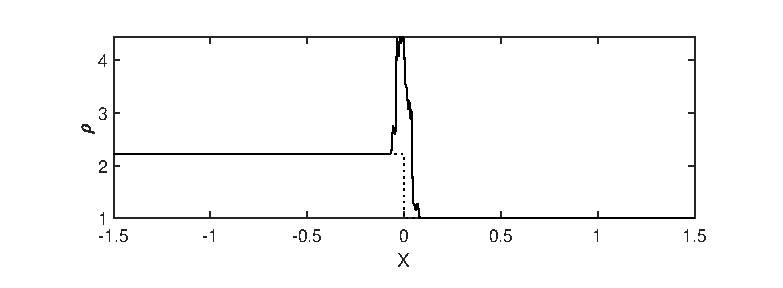
\includegraphics[width=.75\textwidth]{2.1LW.eps}
    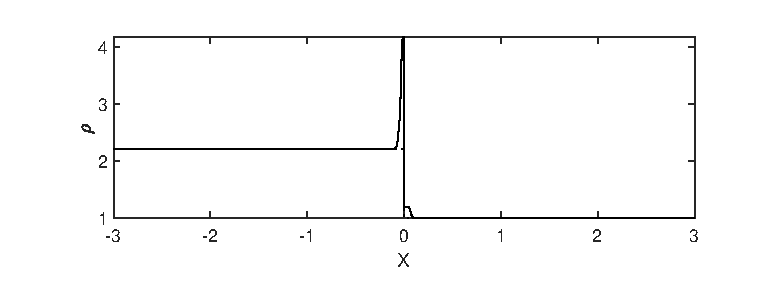
\includegraphics[width=.75\textwidth]{2.1Upwind.eps}
    \caption{较弱慢激波下密度$\rho$分布图. 从上至下对应格式LW,Upwind.虚线是初始分布,实线是时刻$t=0.1$时的分布。}
    \label{fig:2.1m}
\end{figure}
\begin{figure}[H]
    \centering
    \includegraphics[width=.75\textwidth]{2.3LW.eps}
    \includegraphics[width=.75\textwidth]{2.3Up.eps}
    \caption{强激波下密度$\rho$分布图.从上至下对应格式LW,Upwind.虚线是初始分布,实线是时刻$t=1.6$时的分布。}
    \label{fig:2.3m}
\end{figure}
\par
于是分别对较弱的激波采取Upwind格式进行计算,而对强激波采取LW格式进行计算。
\section{数值计算结果}
\subsection{较弱的激波}
对于较弱的快激波初值条件为:
\begin{align}
W_L &= \left[\begin{array}{cccccc}
2.121,
4.981,
-13.27,
-0.163,
-0.6521,
2.572,
10.29
\end{array}\right]^T,
\nonumber\\
W_R &= \left[\begin{array}{ccccccc}
1,
1,
-15.3,
0,
0,
1,
4
\end{array}\right]^T. \label{Eqn:WFast}
\end{align}
\par
我们取Courant系数为0.011,时空网格分别为3001、1001 (强激波计算也沿用此设定). 简单估算此时激波面移动速度接近匀速且沿着$x$轴负向,大小约为11.32;较为显著的特点是相对激波面坐标处,波前后的物理量的值保持不变. 后续时刻计算结果如下图~\ref{fig:2.1mix}所示.
\begin{figure}[H]
    \centering
    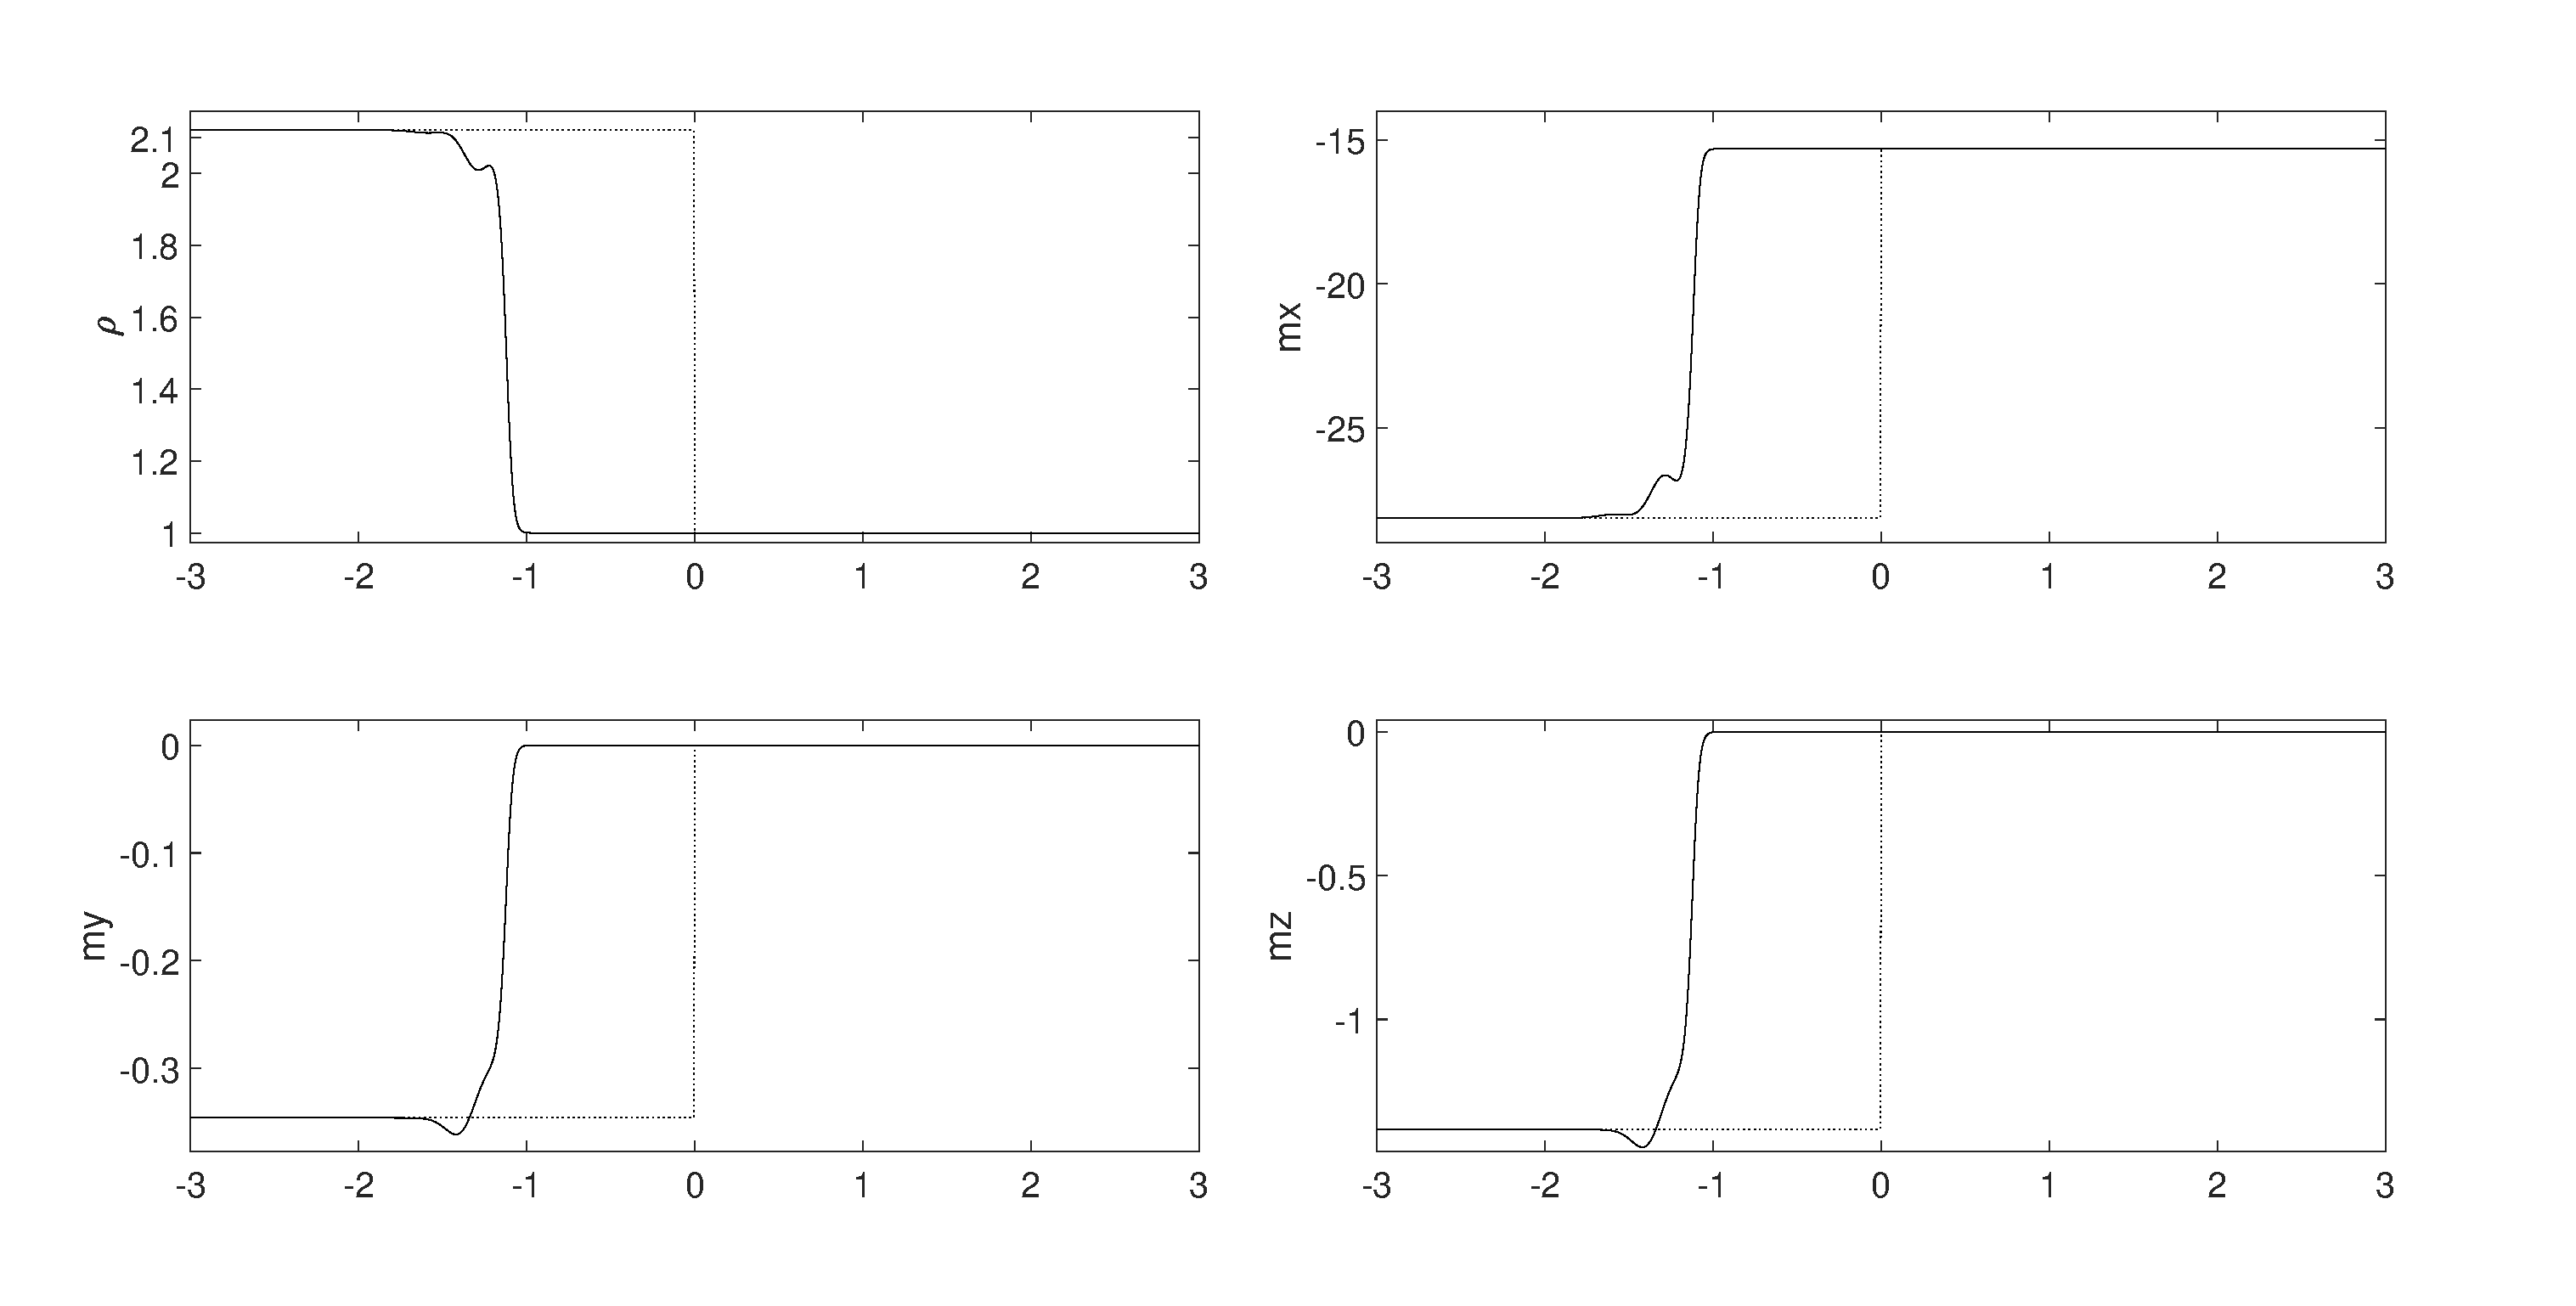
\includegraphics[width=.75\textwidth]{2.1Up1.eps}
    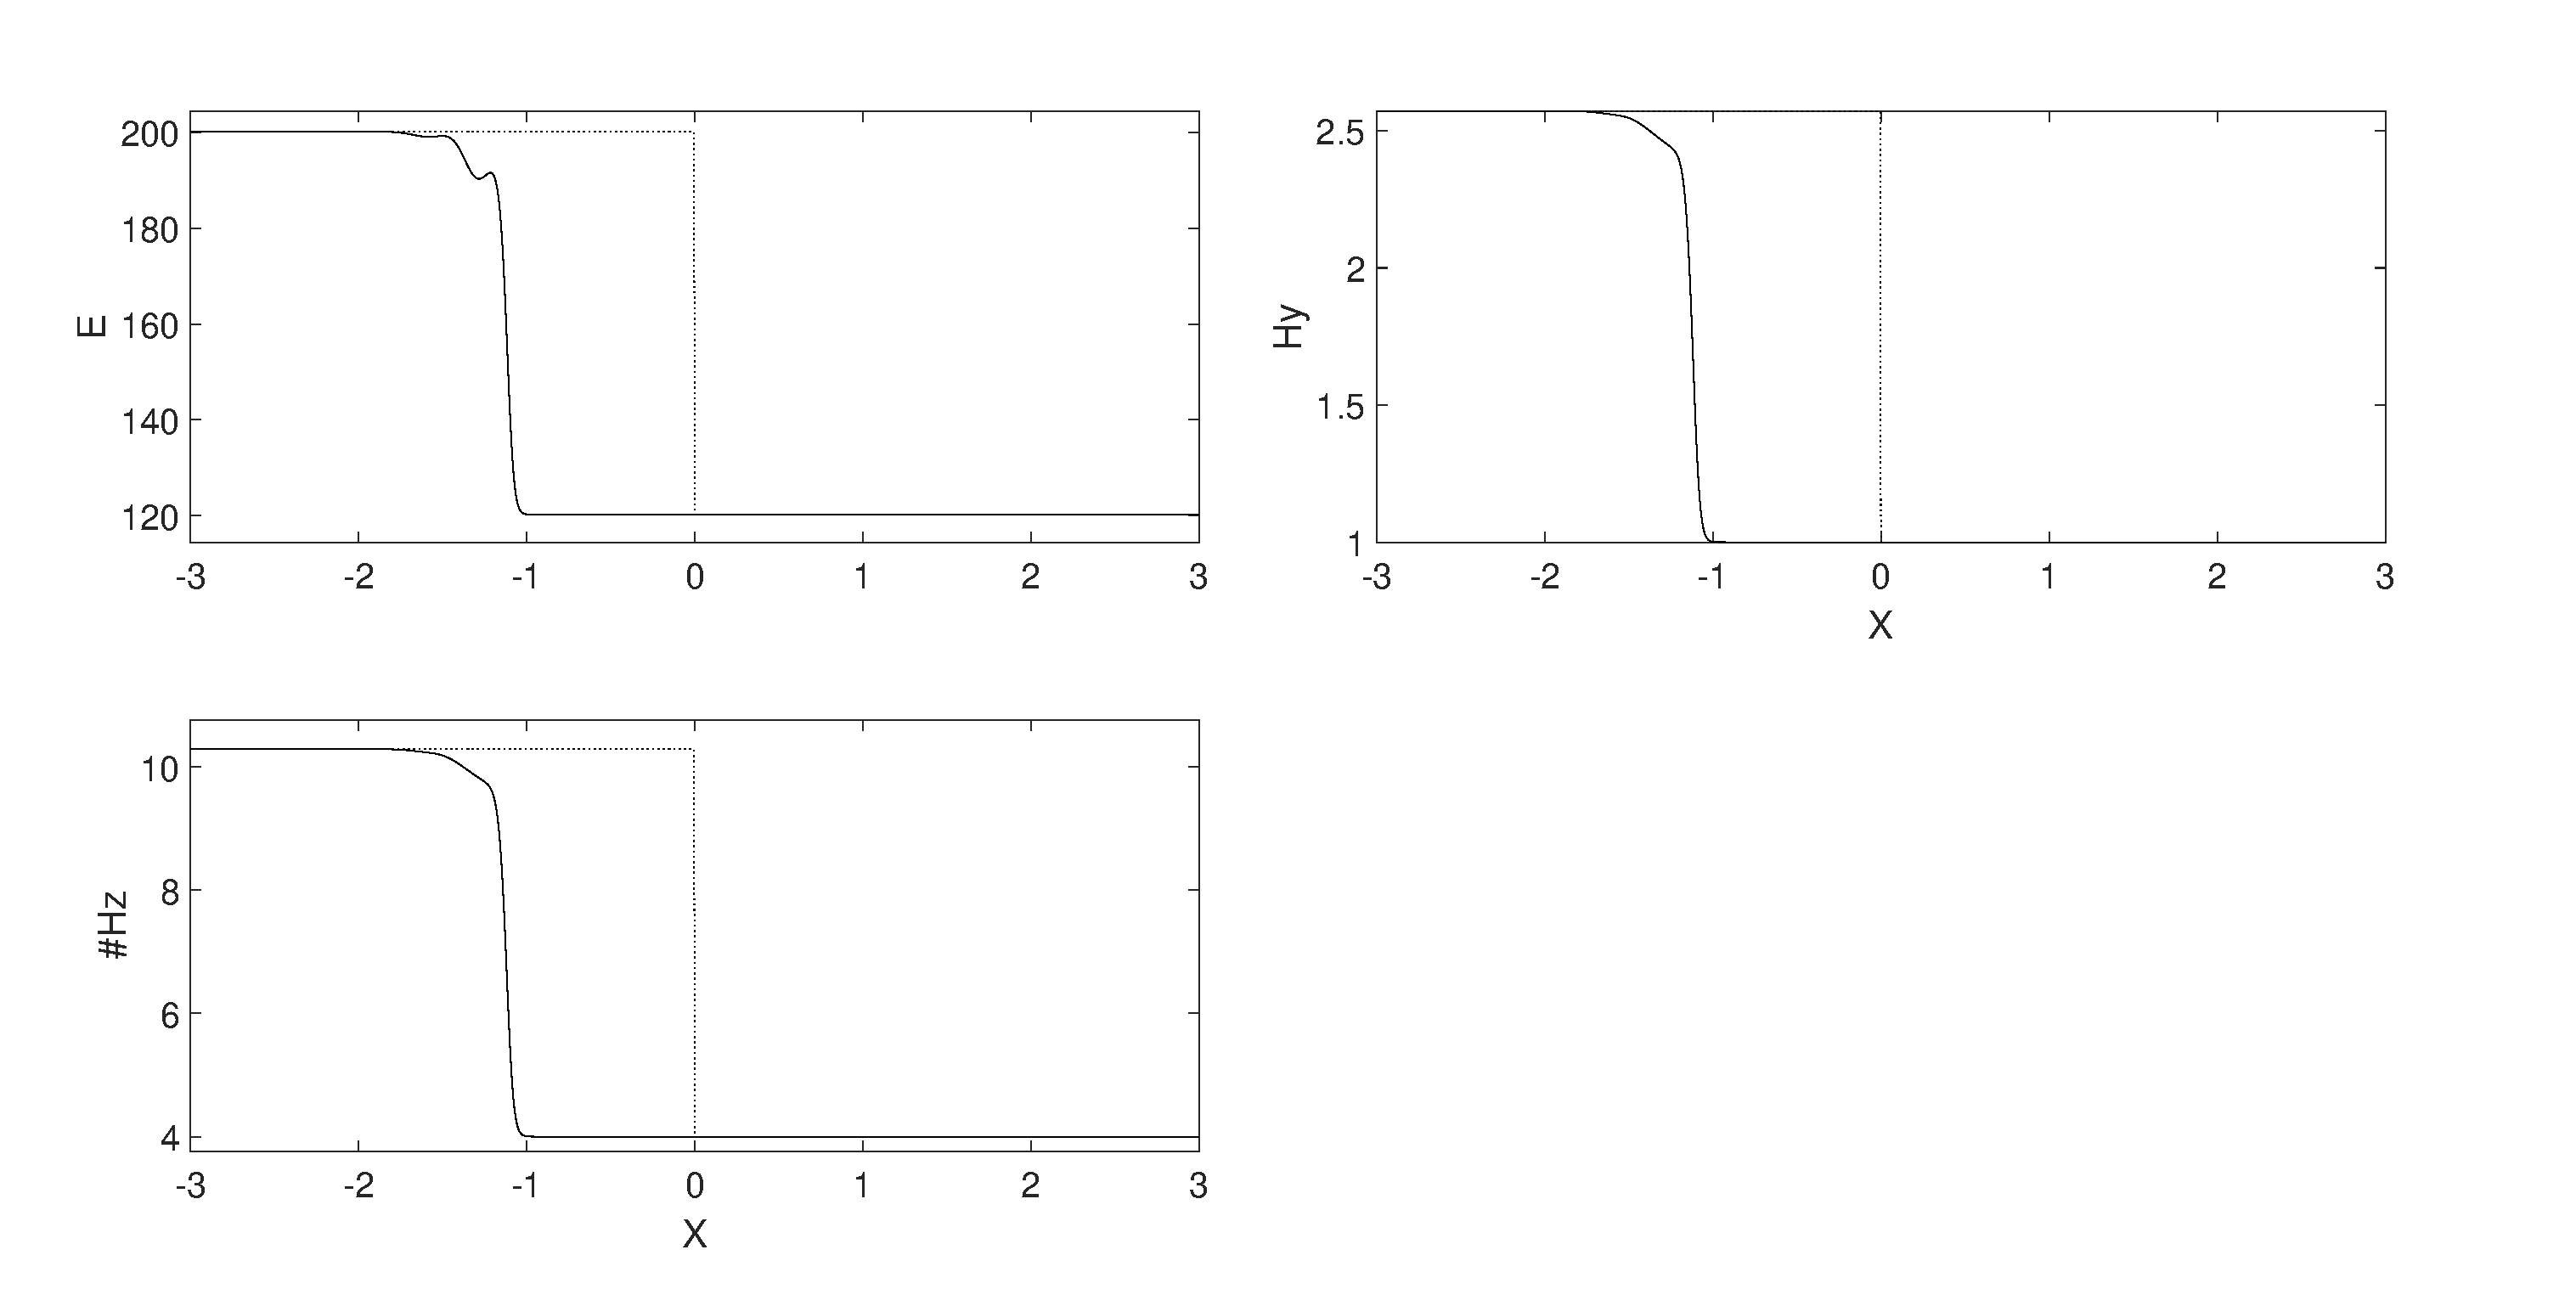
\includegraphics[width=.75\textwidth]{2.1Up2.eps}
    \caption{较弱的快激波下各物理量分布图. 其中$\rho$代表密度,$m$代表动量,$E$代表能量,$H$代表磁场强度.  虚线是初始分布,实线是时刻$t=0.1$时的分布.}
    \label{fig:2.1mix}
\end{figure}
\par
对比Assign4中使用TVD格式计算的结果,显然迎风格式作为精度较低的格式在激波面后附近的位置会有相对明显的耗散.
\subsection{一维MHD快激波}
对于Assign4中2.2节所述强的快激波初值条件为:
\begin{align}
W_L &= \left[\begin{array}{cccccc}
3.896,
305.9,
0,
-0.058,
-0.226,
3.951,
15.8
\end{array}\right]^T,
\nonumber\\
W_R &= \left[\begin{array}{ccccccc}
1,
1,
-15.3,
0,
0,
1,
4
\end{array}\right]^T.\label{Eqn:Fast}
\end{align}
\par
后续时刻计算结果如图~\ref{fig:2.2mix}所示。可以简单估算此时激波面的移动速度接近匀速且沿着$x$轴正向,大小约为5.48.可以注意到,LW格式所展现出的数值振荡性质在图~\ref{fig:2.2mix}中第二行my,mz图像的波前$x=0.3$的位置附近较为明显,但最大振荡幅值不会超过真实值的6\%.
\begin{figure}[H]
    \centering
    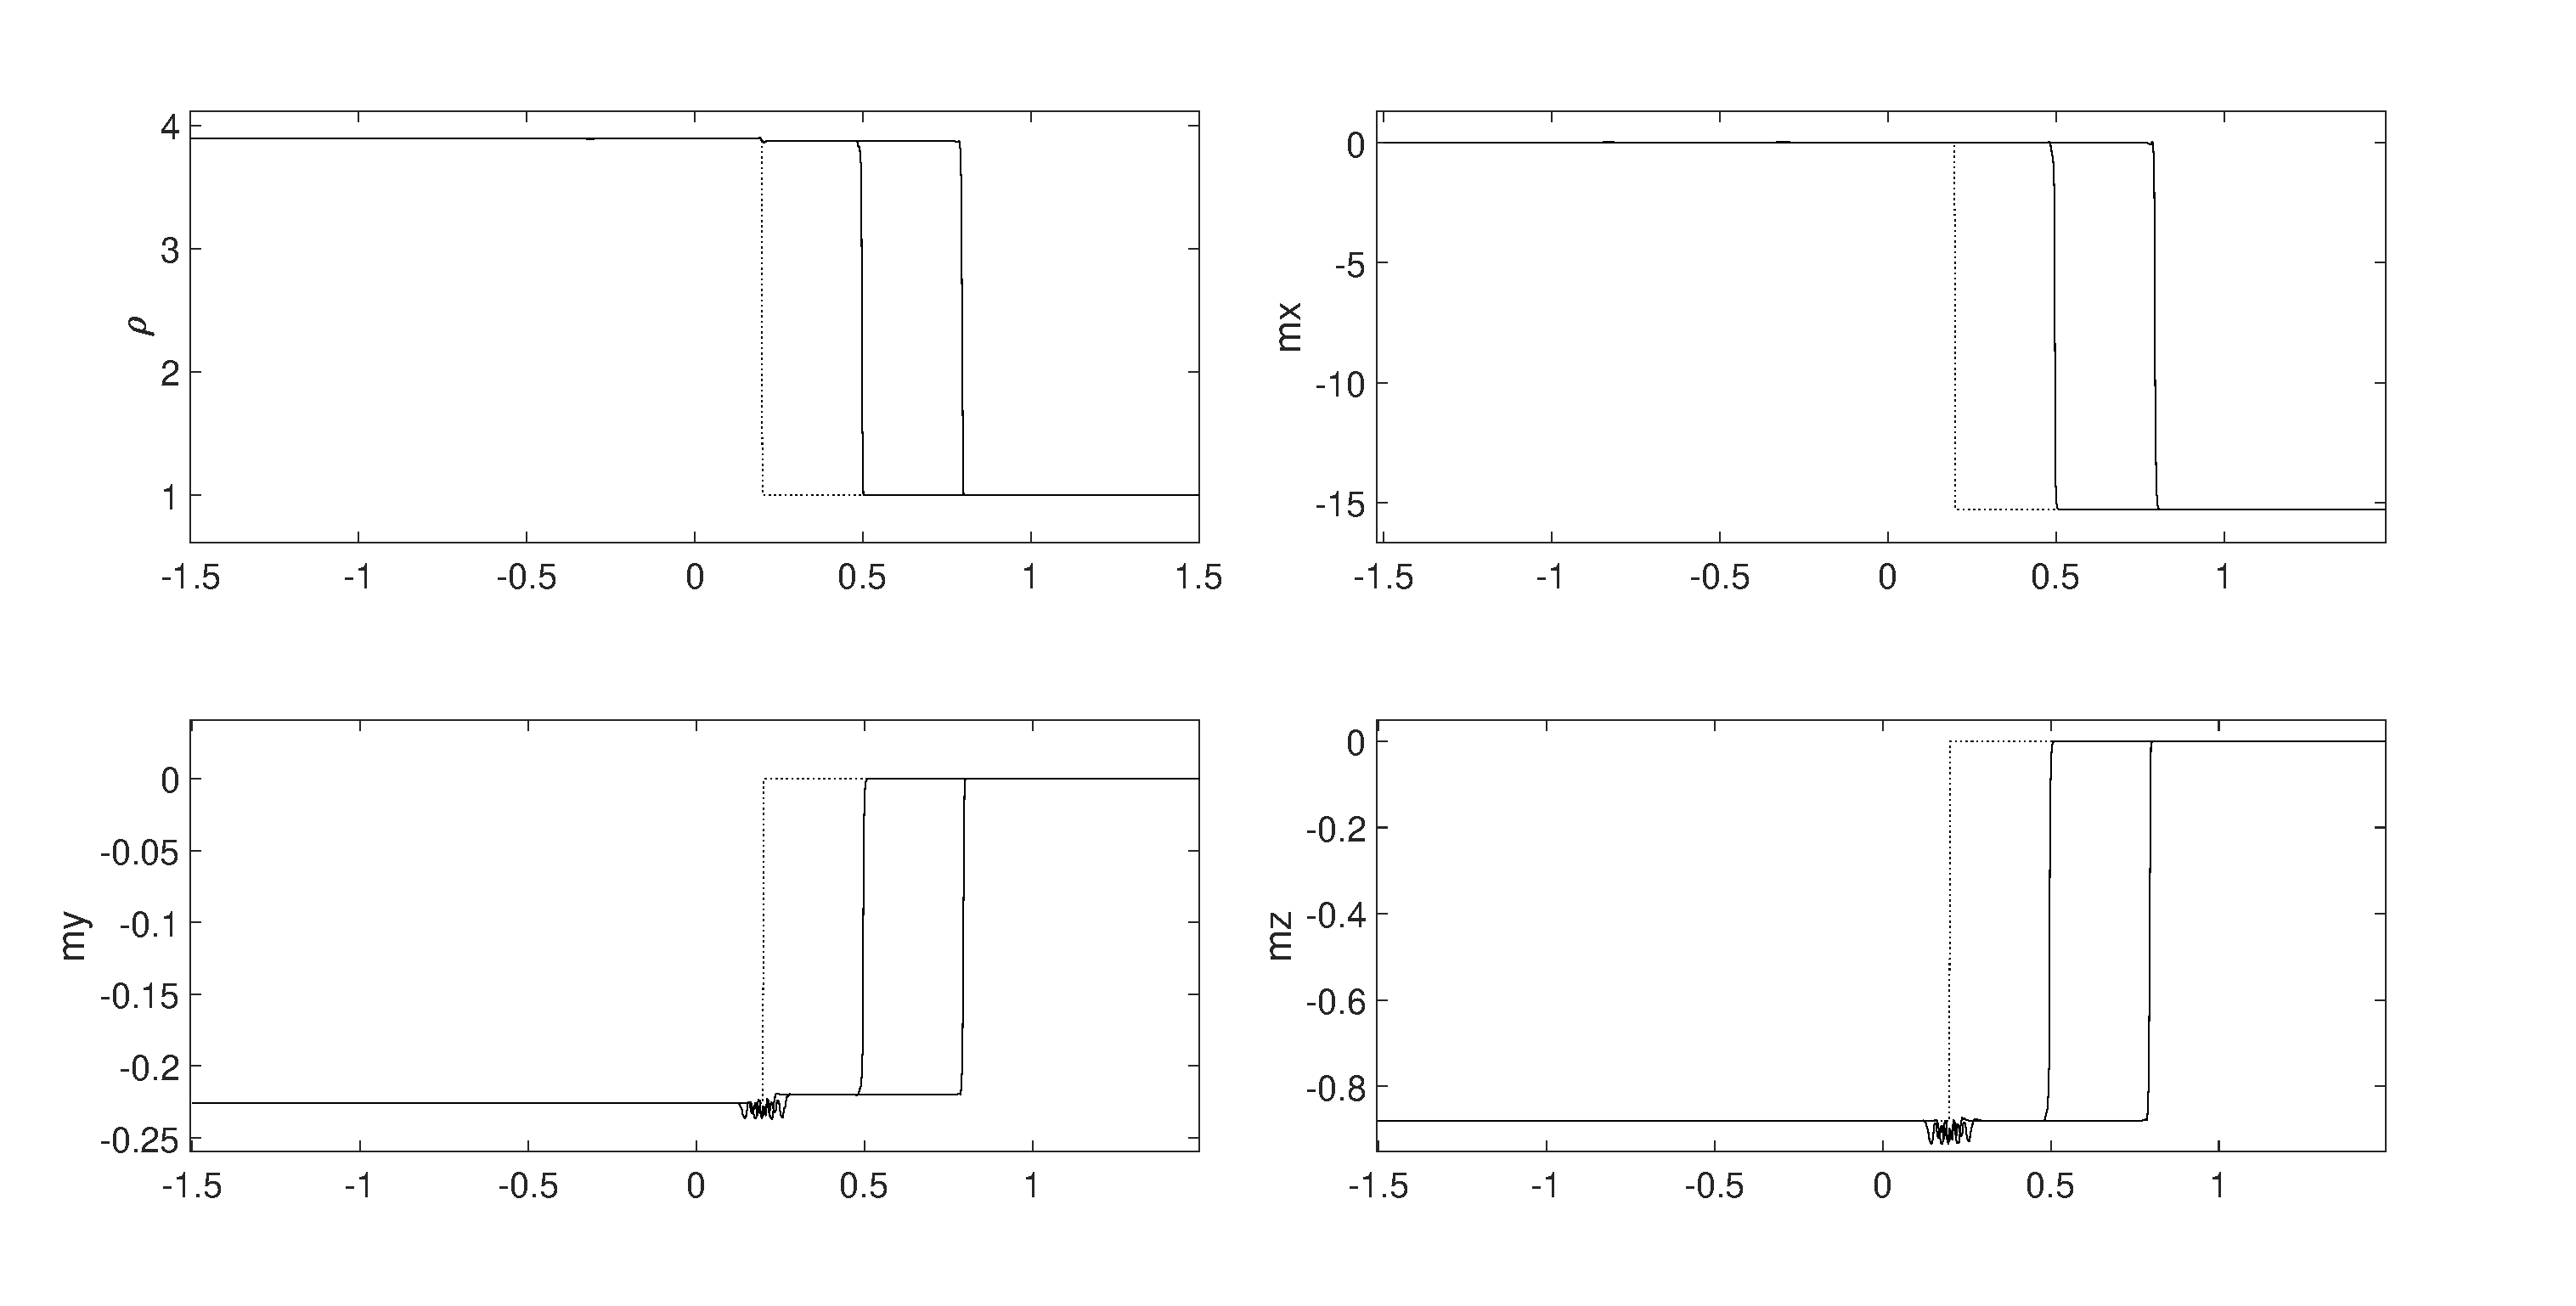
\includegraphics[width=.75\textwidth]{2.2LW1.eps}
    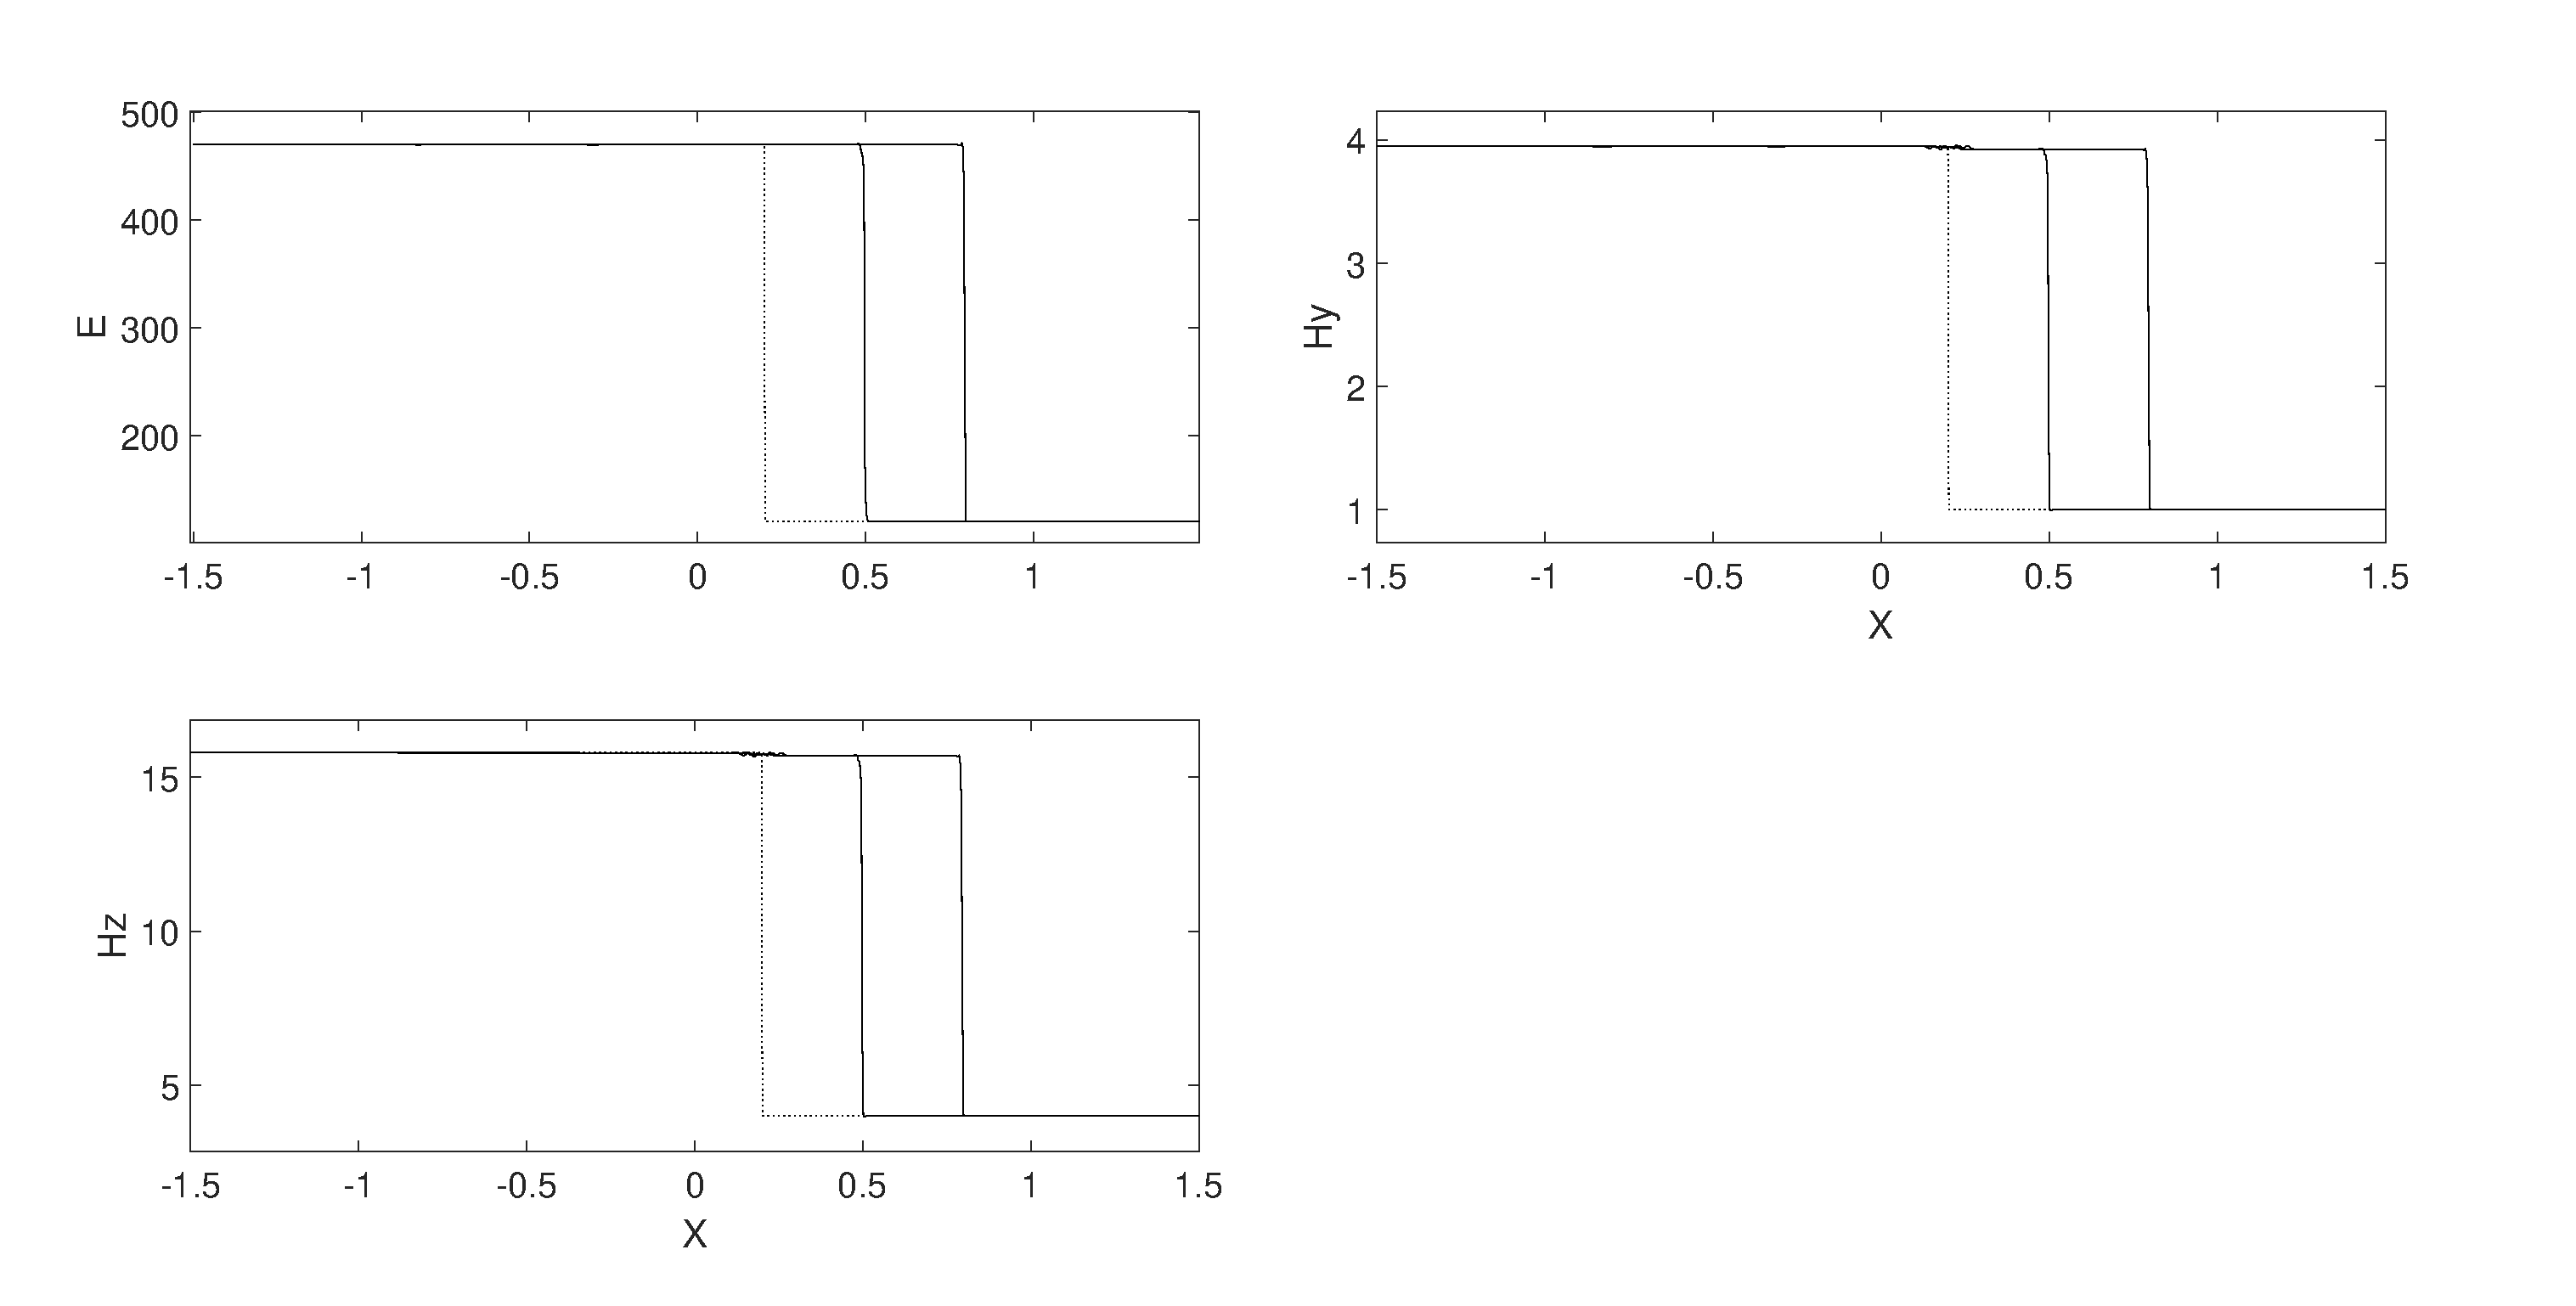
\includegraphics[width=.75\textwidth]{2.2LW2.eps}
    \caption{Assign4中2.2节所述强激波下各物理量分布图. 其中$\rho$代表密度,$m$代表动量,$E$代表能量,$H$代表磁场强度.虚线是初始分布,实线从左至右分别是时刻$t=0.05, 0.1$时的分布。}
    \label{fig:2.2mix}
\end{figure}
\subsection{一维 MHD 慢激波}
对于Assign4中2.3节所述强的慢激波初值条件为:
\begin{align}
W_L &= \left[\begin{array}{ccccccc}
3.108,
1.4336,
0,
0.2633,
0.2633,
0.1,
0.1
\end{array}\right]^T,
\nonumber\\
W_R &= \left[\begin{array}{ccccccc}
1,
0.1,
-0.9225,
0,
0,
1,
1
\end{array}\right]^T.\label{Eqn:Slow}
\end{align}
\par
后续时刻计算结果如下图~\ref{fig:2.3mix}所示。可以简单估算此时激波面的移动速度接近匀速,大小约为0.461.
\begin{figure}[H]
    \centering
    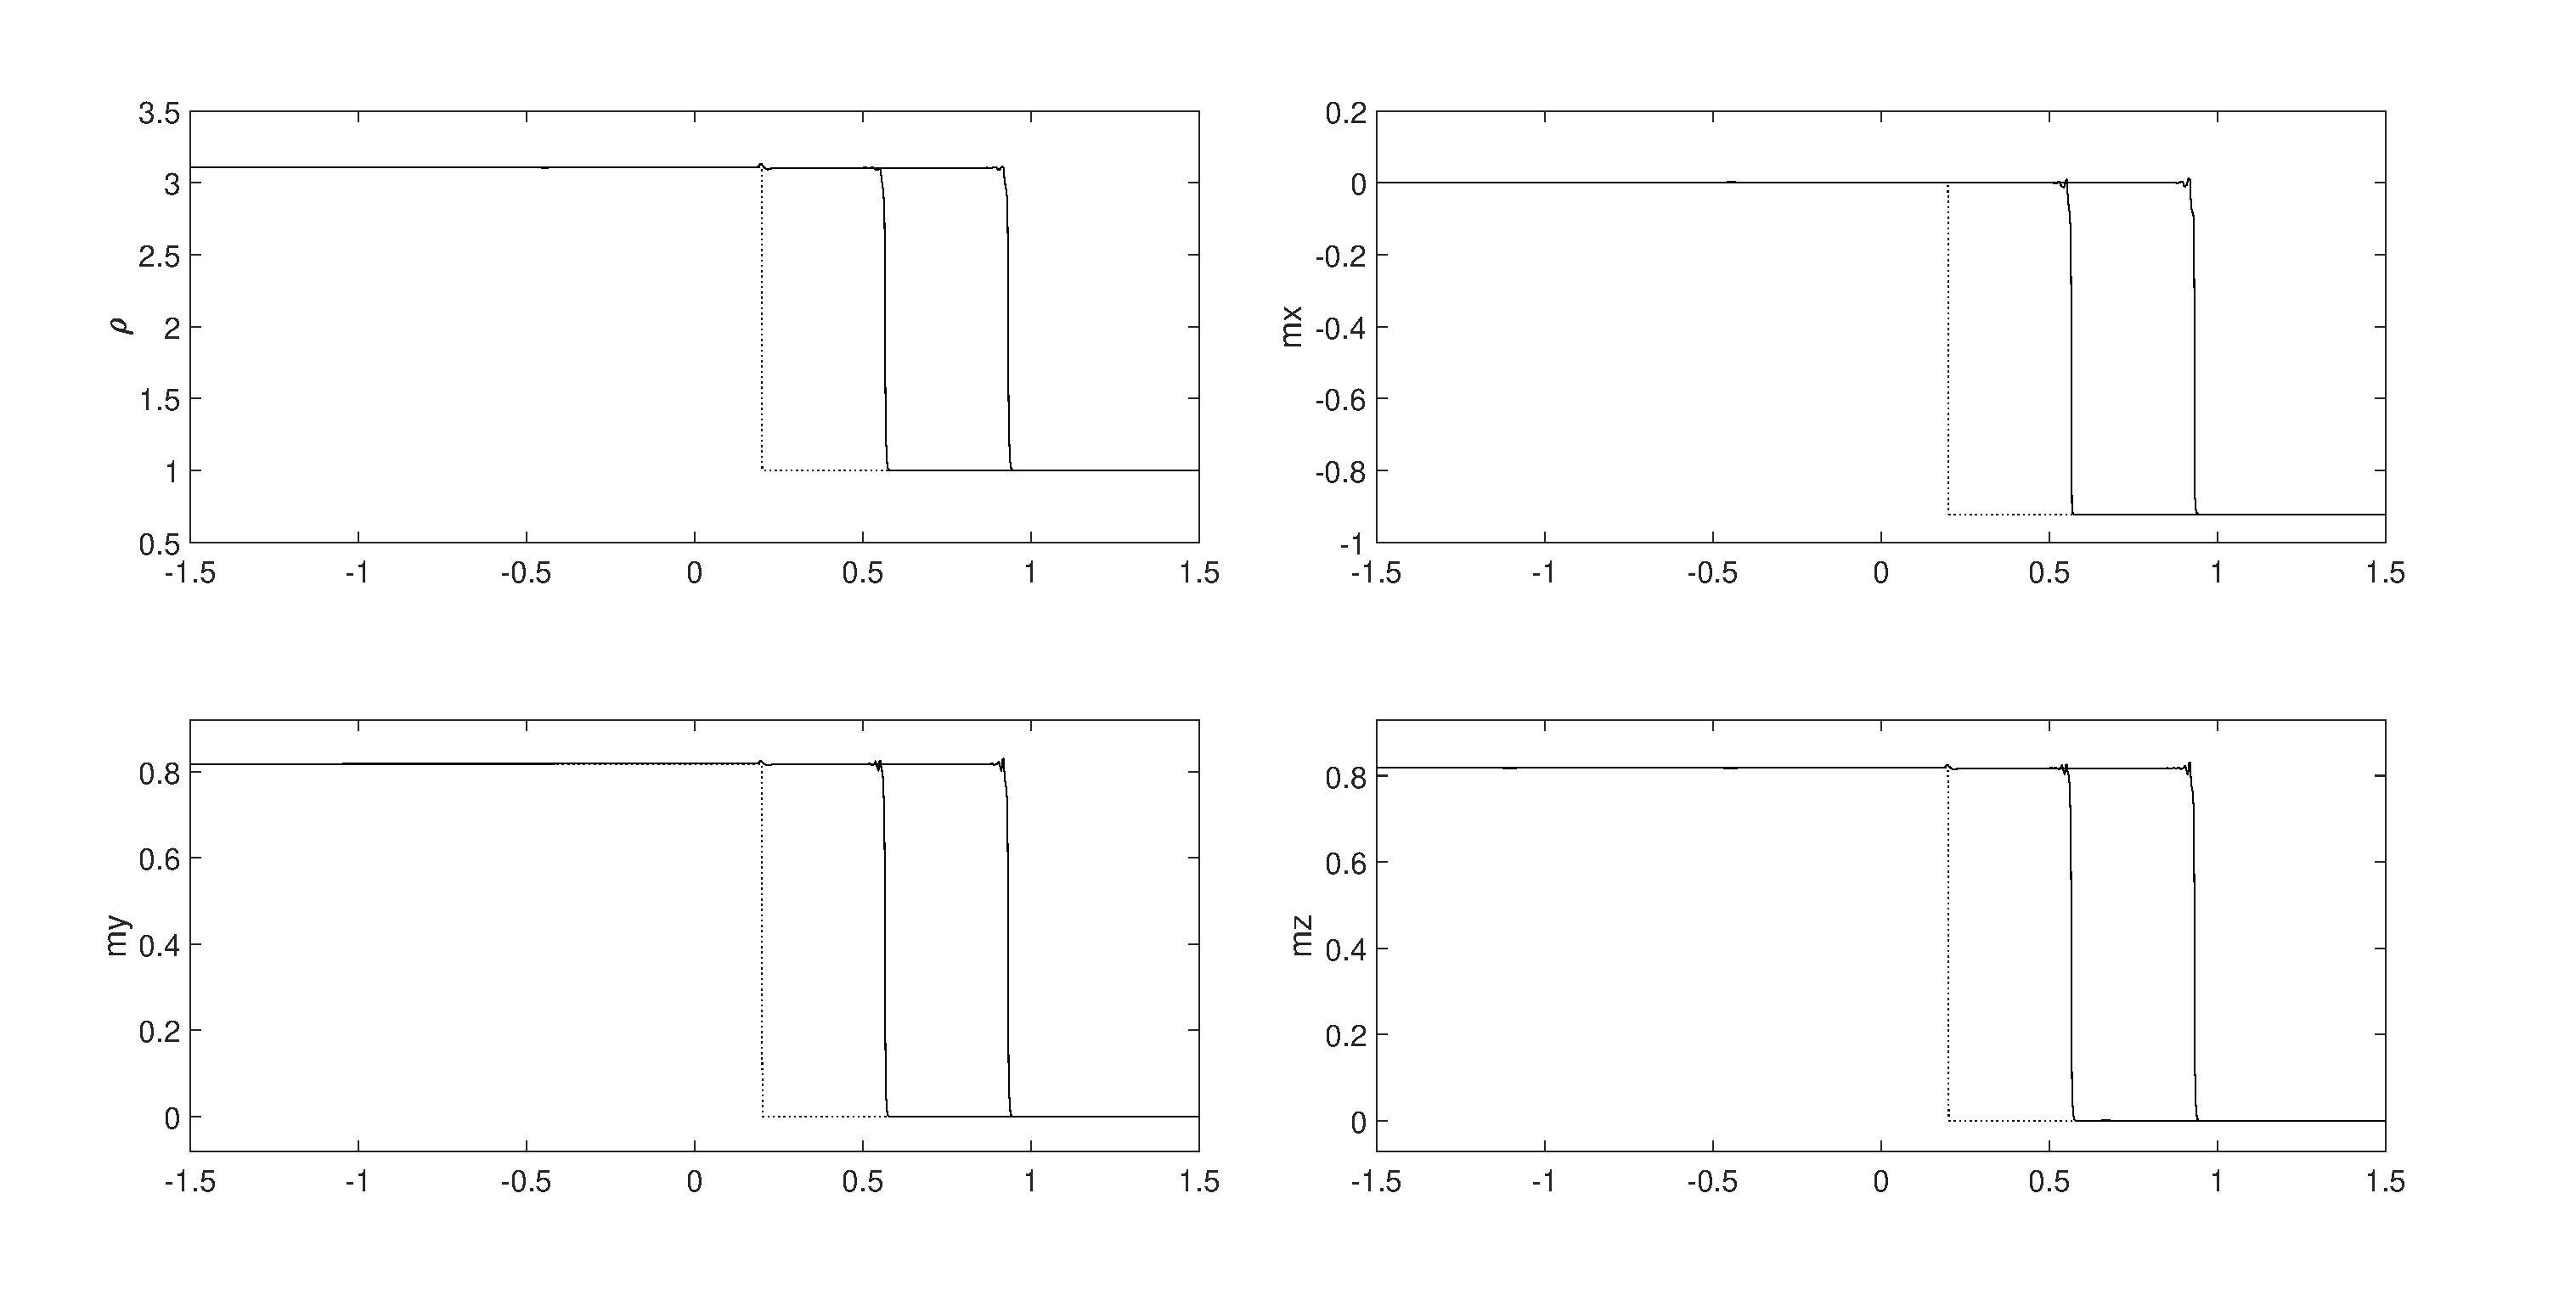
\includegraphics[width=.75\textwidth]{2.3LW1.eps}
    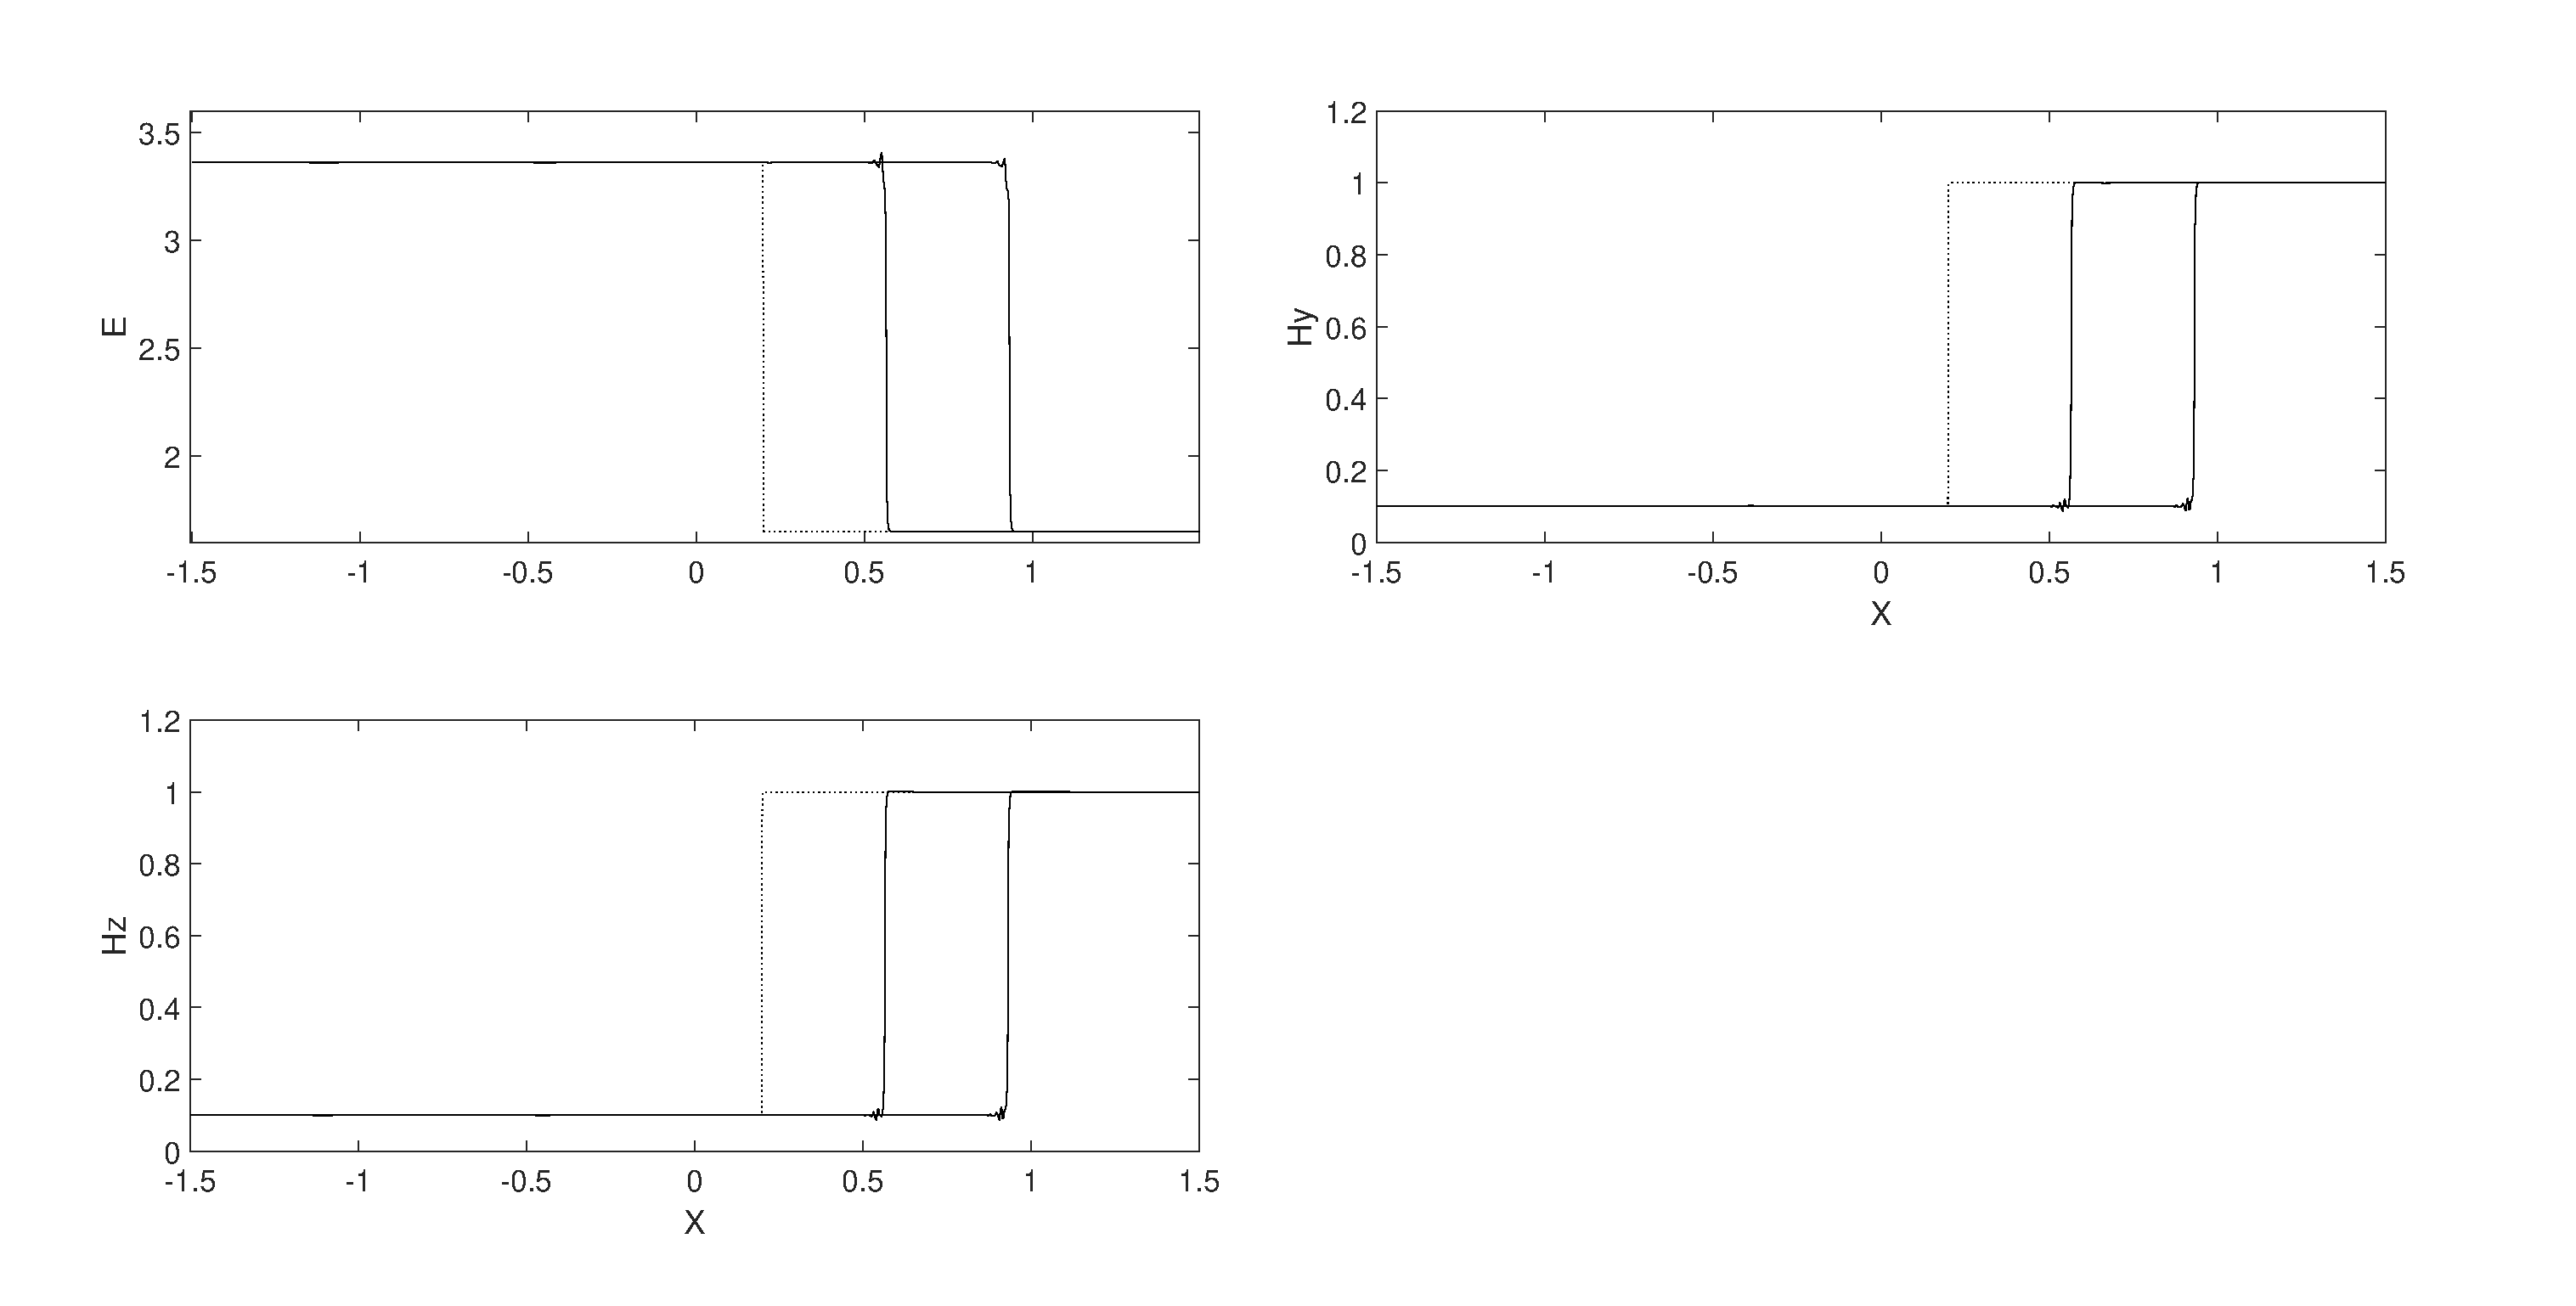
\includegraphics[width=.75\textwidth]{2.3LW2.eps}
    \caption{Asign4中2.3节所述强激波下各物理量分布图.其中$\rho$代表密度,$m$代表动量,$E$代表能量,$H$代表磁场强度. 虚线是初始分布,实线从左至右分别是时刻$t=0.8, 1.6$时分布.}
    \label{fig:2.3mix}
\end{figure}
\section{分工说明}

蓝翔完成了数值格式的计算,蓝翔、苏镇波、康樨共同完成$\rm\LaTeX$的整理排版,以及校验.

\section{附件}

\begin{enumerate}
\item
MHD\_Group10.tex--本报告 \LaTeX 文件
\item
MHD\_Group10.pdf--本报告 PDF 输出文件
\item
Reference.bib--本报告参考文献
\item
code\_combination.txt--计算、绘图代码
\item
2.1LW.eps--图~\ref{fig:2.1m}的eps文件,由Matlab绘制
\item
2.1Up.eps--图~\ref{fig:2.1m}的eps文件,由Matlab绘制
\item
2.3LW.eps--图~\ref{fig:2.3m}的eps文件,由Matlab绘制
\item
2.3Up.eps--图~\ref{fig:2.3m}的eps文件,由Matlab绘制
\item
2.1Up1.eps--图~\ref{fig:2.1mix}的eps文件,由Matlab绘制
\item
2.1Up2.eps--图~\ref{fig:2.1mix}的eps文件,由Matlab绘制
\item
2.2LW1.eps--图~\ref{fig:2.2mix}的eps文件,由Matlab绘制
\item
2.2LW2.eps--图~\ref{fig:2.2mix}的eps文件,由Matlab绘制
\item
2.3LW1.eps--图~\ref{fig:2.3mix}的eps文件,由Matlab绘制
\item
2.3LW2.eps--图~\ref{fig:2.3mix}的eps文件,由Matlab绘制
\end{enumerate}
% 以下两行是中文文献国家标准的格式, 如果安装了这两个格式, 建议使用它们
% \bibliographystyle{gbt7714-author-year}
% \bibliographystyle{gbt7714-numerical}
%

%\bibliographystyle{unsrt}
\bibliographystyle{apalike}
\bibliography{References}

%\begin{thebibliography}{1}
%
%\bibitem{Diver2001}
%Declan~A. Diver.
%\newblock {\em A plasma formulary for physics, technology and astrophysics}.
%\newblock Wiley VCH, 1st edition, 2001.
%
%\bibitem{Jeffrey1964}
%A.~Jeffrey and T.~Taniuti.
%\newblock {\em Non-Linear Wave Propagation with Applications to Physics and
%  Magnetohydrodynamics}, volume~9 of {\em Mathematics in Science and
%  Engineering - A Series of Monographs and Textbooks}.
%\newblock Academic Press, New York / London, 1964.

%\end{thebibliography}

\end{document}
